\begin{exercise}[Payoff diagrams for elementary option strategies]
Plot the terminal payoffs of the listed strategies.  The diagrams below are
terminal payoffs before taking account of option premiums.
\end{exercise}

\begin{solution}
Write \(x=S_T\).  The terminal payoff of each strategy is the sum of its
component terminal payoffs; option premiums are paid at inception and are
therefore not included in the maturity payoff diagrams.

\[
\begin{array}{ll}
\text{short stock + two calls at }K:
  & -x+2\pos{x-K},\\[0.3em]
\text{long call + long put at }K:
  & \pos{x-K}+\pos{K-x}=|x-K|,\\[0.3em]
\text{strip: one call + two puts at }K:
  & \pos{x-K}+2\pos{K-x},\\[0.3em]
\text{strap: two calls + one put at }K:
  & 2\pos{x-K}+\pos{K-x},\\[0.3em]
\text{strangle: call at }K_1\text{ + put at }K_2:
  & \pos{x-K_1}+\pos{K_2-x},\\[0.3em]
\text{bull spread, }K_1<K_2:
  & \pos{x-K_1}-\pos{x-K_2},\\[0.3em]
\text{bear spread, }K_1<K_2:
  & \pos{x-K_2}-\pos{x-K_1},\\[0.3em]
\text{butterfly, }K_1<K_2<K_3:
  & \pos{x-K_1}-2\pos{x-K_2}+\pos{x-K_3}.
\end{array}
\]
The first strategy is a straddle up to the deterministic cash shift \(K\):
by put-call parity at maturity,
\[
  -x+2\pos{x-K}+K=\pos{x-K}+\pos{K-x}=|x-K|.
\]
The usual long straddle is the second strategy: it pays when the underlying
finishes far away from the common strike in either direction.

\begin{center}
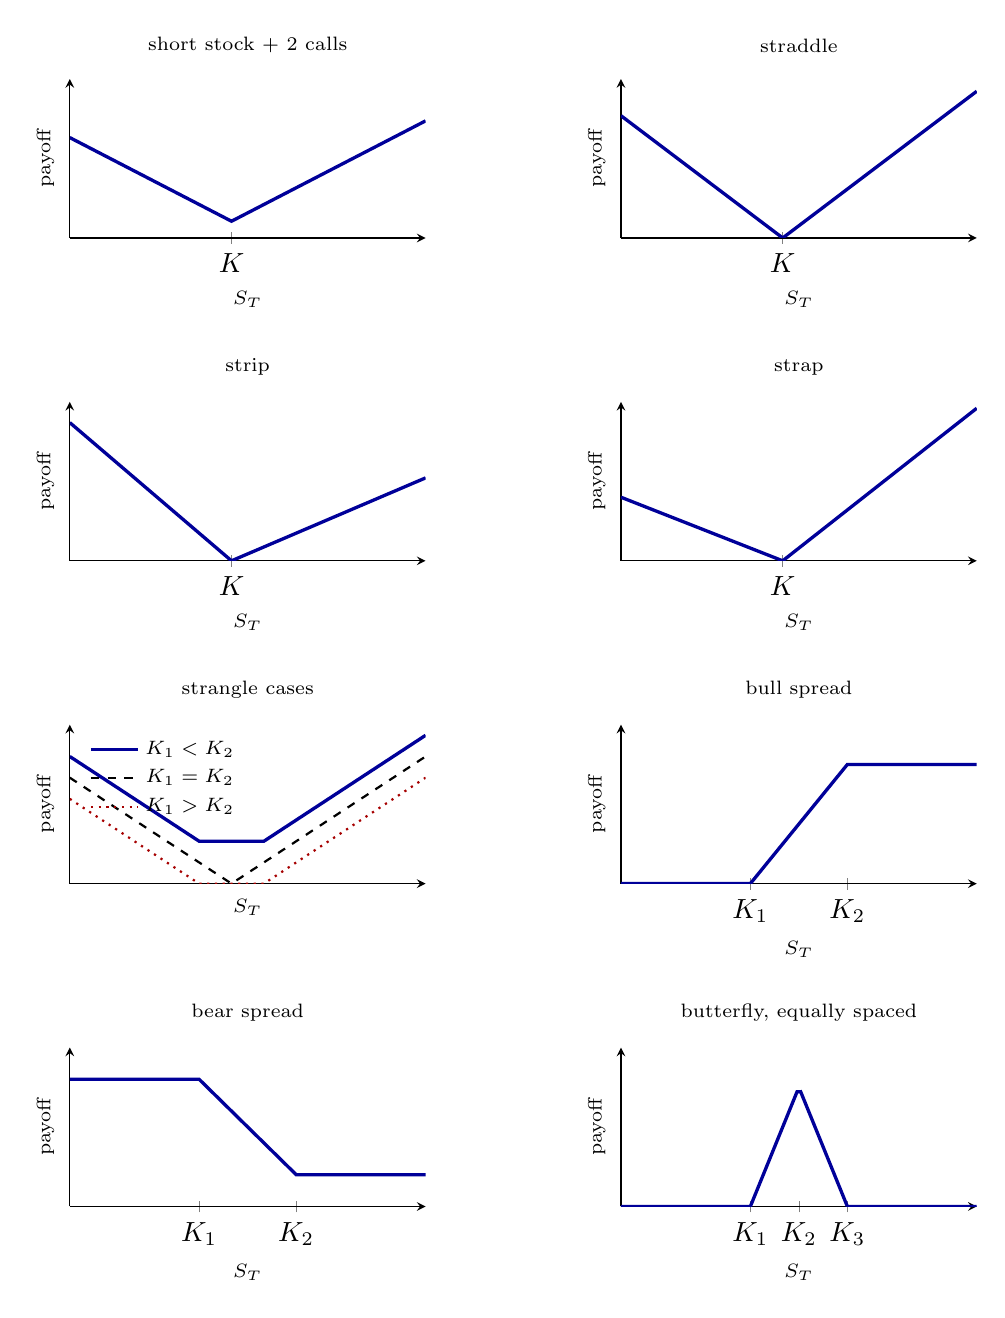
\begin{tikzpicture}
  \begin{scope}
  \begin{axis}[
    width=6.1cm,height=3.6cm,axis lines=left,xmin=0,xmax=2.2,ymin=-1.2,ymax=0.7,
    xtick={1},xticklabels={\(K\)},ytick=\empty,title={\scriptsize short stock + \(2\) calls},
    xlabel={\scriptsize \(S_T\)},ylabel={\scriptsize payoff}
  ]
    \addplot[blue!60!black,very thick,domain=0:2.2,samples=100] {2*max(x-1,0)-x};
  \end{axis}
  \end{scope}

  \begin{scope}[xshift=7cm]
  \begin{axis}[
    width=6.1cm,height=3.6cm,axis lines=left,xmin=0,xmax=2.2,ymin=0,ymax=1.3,
    xtick={1},xticklabels={\(K\)},ytick=\empty,title={\scriptsize straddle},
    xlabel={\scriptsize \(S_T\)},ylabel={\scriptsize payoff}
  ]
    \addplot[blue!60!black,very thick,domain=0:2.2,samples=100] {abs(x-1)};
  \end{axis}
  \end{scope}

  \begin{scope}[yshift=-4.1cm]
  \begin{axis}[
    width=6.1cm,height=3.6cm,axis lines=left,xmin=0,xmax=2.2,ymin=0,ymax=2.3,
    xtick={1},xticklabels={\(K\)},ytick=\empty,title={\scriptsize strip},
    xlabel={\scriptsize \(S_T\)},ylabel={\scriptsize payoff}
  ]
    \addplot[blue!60!black,very thick,domain=0:2.2,samples=100] {max(x-1,0)+2*max(1-x,0)};
  \end{axis}
  \end{scope}

  \begin{scope}[xshift=7cm,yshift=-4.1cm]
  \begin{axis}[
    width=6.1cm,height=3.6cm,axis lines=left,xmin=0,xmax=2.2,ymin=0,ymax=2.5,
    xtick={1},xticklabels={\(K\)},ytick=\empty,title={\scriptsize strap},
    xlabel={\scriptsize \(S_T\)},ylabel={\scriptsize payoff}
  ]
    \addplot[blue!60!black,very thick,domain=0:2.2,samples=100] {2*max(x-1,0)+max(1-x,0)};
  \end{axis}
  \end{scope}

  \begin{scope}[yshift=-8.2cm]
  \begin{axis}[
    width=6.1cm,height=3.6cm,axis lines=left,xmin=0,xmax=2.2,ymin=0,ymax=1.5,
    xtick=\empty,ytick=\empty,
    title={\scriptsize strangle cases},xlabel={\scriptsize \(S_T\)},ylabel={\scriptsize payoff},
    legend style={font=\scriptsize,draw=none,fill=none,at={(0.03,0.97)},anchor=north west}
  ]
    \addplot[blue!60!black,very thick,domain=0:2.2,samples=100] {max(x-0.8,0)+max(1.2-x,0)};
    \addlegendentry{\(K_1<K_2\)}
    \addplot[black,thick,dashed,domain=0:2.2,samples=100] {abs(x-1)};
    \addlegendentry{\(K_1=K_2\)}
    \addplot[red!65!black,thick,dotted,domain=0:2.2,samples=100] {max(x-1.2,0)+max(0.8-x,0)};
    \addlegendentry{\(K_1>K_2\)}
  \end{axis}
  \end{scope}

  \begin{scope}[xshift=7cm,yshift=-8.2cm]
  \begin{axis}[
    width=6.1cm,height=3.6cm,axis lines=left,xmin=0,xmax=2.2,ymin=0,ymax=0.8,
    xtick={0.8,1.4},xticklabels={\(K_1\),\(K_2\)},ytick=\empty,title={\scriptsize bull spread},
    xlabel={\scriptsize \(S_T\)},ylabel={\scriptsize payoff}
  ]
    \addplot[blue!60!black,very thick,domain=0:2.2,samples=100] {max(x-0.8,0)-max(x-1.4,0)};
  \end{axis}
  \end{scope}

  \begin{scope}[yshift=-12.3cm]
  \begin{axis}[
    width=6.1cm,height=3.6cm,axis lines=left,xmin=0,xmax=2.2,ymin=-0.8,ymax=0.2,
    xtick={0.8,1.4},xticklabels={\(K_1\),\(K_2\)},ytick=\empty,title={\scriptsize bear spread},
    xlabel={\scriptsize \(S_T\)},ylabel={\scriptsize payoff}
  ]
    \addplot[blue!60!black,very thick,domain=0:2.2,samples=100] {max(x-1.4,0)-max(x-0.8,0)};
  \end{axis}
  \end{scope}

  \begin{scope}[xshift=7cm,yshift=-12.3cm]
  \begin{axis}[
    width=6.1cm,height=3.6cm,axis lines=left,xmin=0,xmax=2.2,ymin=0,ymax=0.4,
    xtick={0.8,1.1,1.4},xticklabels={\(K_1\),\(K_2\),\(K_3\)},ytick=\empty,title={\scriptsize butterfly, equally spaced},
    xlabel={\scriptsize \(S_T\)},ylabel={\scriptsize payoff}
  ]
    \addplot[blue!60!black,very thick,domain=0:2.2,samples=100] {max(x-0.8,0)-2*max(x-1.1,0)+max(x-1.4,0)};
  \end{axis}
  \end{scope}
\end{tikzpicture}
\end{center}

For the butterfly, the right tail is
\[
  (x-K_1)-2(x-K_2)+(x-K_3)=2K_2-K_1-K_3,
  \qquad x\ge K_3.
\]
Thus the usual tent-shaped butterfly with zero right tail requires equally
spaced strikes, i.e. \(K_2=(K_1+K_3)/2\).  Without this spacing condition the
payoff becomes a non-zero constant for \(x\ge K_3\).
\end{solution}
